\documentclass[finnish,colorlinks,headings=normal,parskip=half,footsepline]{scrartcl}

\usepackage[utf8]{inputenc}
\usepackage[T1]{fontenc}
\usepackage{libertine,babel,setspace,ragged2e,scrlayer-scrpage,lastpage,geometry,calc,graphicx,wrapfig}
\usepackage[activate=false,stretch=0,letterspace=120]{microtype}
\usepackage{hyperref}

\RaggedRight
\frenchspacing
\setstretch{1.04}
\setkomafont{pageheadfoot}{\scriptsize\sffamily}
\setkomafont{pagenumber}{\scriptsize\sffamily}
\addtokomafont{disposition}{\rmfamily}
\urlstyle{same}
\clearpairofpagestyles
\lofoot*{\lsstyle\MakeUppercase{J.~Suomalainen: insta}}
\rofoot*{\lsstyle SIVU~\pagemark/\pageref{LastPage}}
\newcommand*\GetTextWidth[3][\normalfont]{{#1%
		\settowidth{#2}{abcdefghijklmnopqrstuvwxyz}%
		\setlength{#2}{0.03193#2}%
		\addtolength{#2}{0.44961pt}%
		\setlength{#2}{#3#2}%
		\global#2=#2}}
\newlength\bringhurstwdt
\GetTextWidth{\bringhurstwdt}{70}
\geometry{top=1.5in,bottom=1.75in,textwidth=\bringhurstwdt}
\addtolength{\footskip}{-22pt}

\begin{document}
Janne Suomalainen\\\textsf{insta} (0.9)\\Web"-palvelinohjelmointi Java "=kurssin harjoitustyö\\\today

\section{Sovellus}
Sovellus löytyy osoitteesta \url{https://evening-island-18993.herokuapp.com}. Sovelluksen lähdekoodi löytyy \href{https://github.com/suomja1/insta}{GitHubista} ja sen testaus (versiossa 0.9 ei ole implementoitu yhtään testiä) on automatisoitu \href{https://travis-ci.org/suomja1/insta}{Travis-palvelun} avulla.

\textsf{insta} on pelkistetty kuvapalvelu (vertaa \href{https://www.instagram.com}{Instagram}), jossa käyttäjä pystyy lisäämään, selaamaan sekä kommentoimaan kuvia. Kuvien selaamisen helpottamiseksi kuviin voi lisätä erilaisia tunnisteita (vertaa \emph{hashtag}).

Erilliset tuotanto- ja testausprofiilit sujuvoittavat sovelluksen kehittämistä. \textsf{insta}ssa profiilit on toteutettu erillisillä konfiguraatiotiedostoilla ja Springin tarjoamalla Profile"-annotaatiolla. Käytettävä profiili valitaan sovelluksen main"-luokassa SpringApplication"-luokan setAdditionalProfiles"-metodilla.

\textsf{insta}an tunnistaudutaan käyttäjänimellä ja salasanalla. Kuka tahansa pystyy luomaan käyttäjän kirjautumissivulla.

\begin{wrapfigure}{r}{.5\linewidth-.5\columnsep}
\vspace*{-\intextsep}
\centering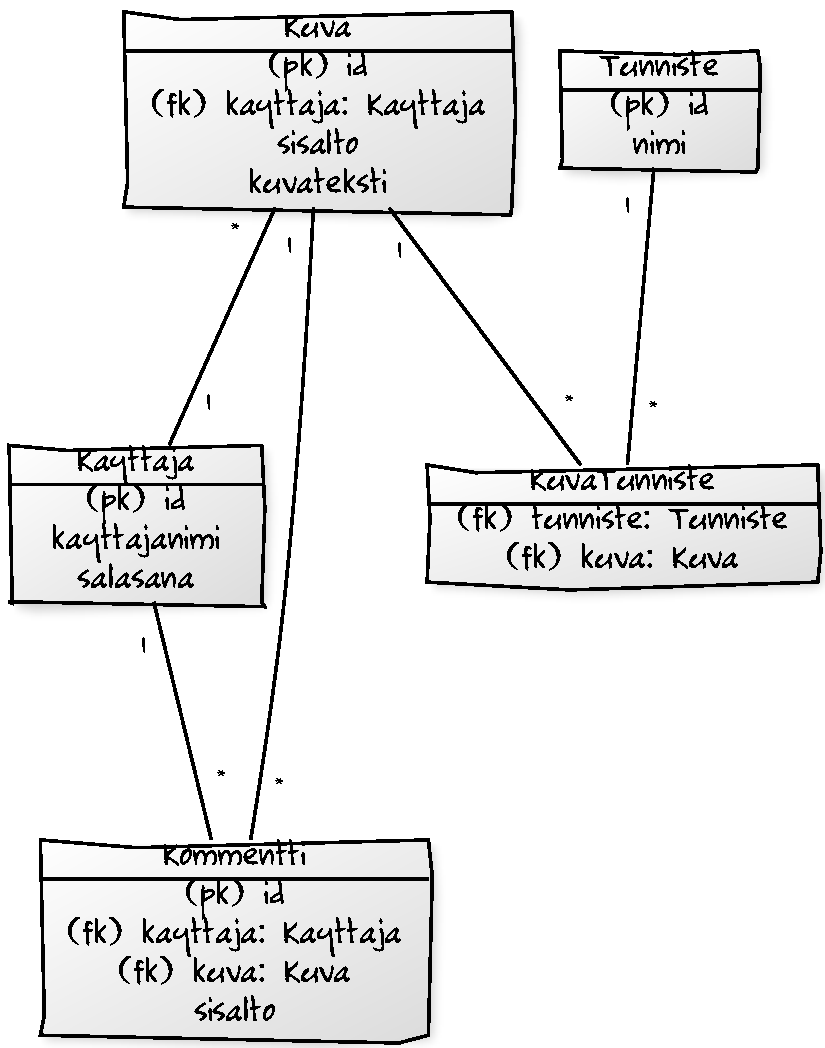
\includegraphics[width=\linewidth]{6424b8c7}
\caption{Tietokantakaavio.}\label{fig:tk}
\end{wrapfigure}

Sovellus käyttää tietokantaa, jossa on yhteensä viisi taulua. Yksi näistä on liitostaulu. Testausprofiilissa käytetään H2 Database "-tietokantaa, joka ladataan muistiin aina sovelluksen käynnistyessä. Tuotantoprofiilissa käytetään Herokun tarjoamaa Postgres"-tietokantaa. Tietokantakaavio on esitetty kuvassa~\ref{fig:tk}.

\section{Keskeisiä käyttötapauksia}
navigointi

syötteiden validointi

\section{Jatkokehitys}
testit

syötteiden validointi

roolit

virheviestit
\end{document}